% Options for packages loaded elsewhere
\PassOptionsToPackage{unicode}{hyperref}
\PassOptionsToPackage{hyphens}{url}
\documentclass[
]{article}
\usepackage{xcolor}
\usepackage[margin=1in]{geometry}
\usepackage{amsmath,amssymb}
\setcounter{secnumdepth}{-\maxdimen} % remove section numbering
\usepackage{iftex}
\ifPDFTeX
  \usepackage[T1]{fontenc}
  \usepackage[utf8]{inputenc}
  \usepackage{textcomp} % provide euro and other symbols
\else % if luatex or xetex
  \usepackage{unicode-math} % this also loads fontspec
  \defaultfontfeatures{Scale=MatchLowercase}
  \defaultfontfeatures[\rmfamily]{Ligatures=TeX,Scale=1}
\fi
\usepackage{lmodern}
\ifPDFTeX\else
  % xetex/luatex font selection
\fi
% Use upquote if available, for straight quotes in verbatim environments
\IfFileExists{upquote.sty}{\usepackage{upquote}}{}
\IfFileExists{microtype.sty}{% use microtype if available
  \usepackage[]{microtype}
  \UseMicrotypeSet[protrusion]{basicmath} % disable protrusion for tt fonts
}{}
\makeatletter
\@ifundefined{KOMAClassName}{% if non-KOMA class
  \IfFileExists{parskip.sty}{%
    \usepackage{parskip}
  }{% else
    \setlength{\parindent}{0pt}
    \setlength{\parskip}{6pt plus 2pt minus 1pt}}
}{% if KOMA class
  \KOMAoptions{parskip=half}}
\makeatother
\usepackage{color}
\usepackage{fancyvrb}
\newcommand{\VerbBar}{|}
\newcommand{\VERB}{\Verb[commandchars=\\\{\}]}
\DefineVerbatimEnvironment{Highlighting}{Verbatim}{commandchars=\\\{\}}
% Add ',fontsize=\small' for more characters per line
\usepackage{framed}
\definecolor{shadecolor}{RGB}{248,248,248}
\newenvironment{Shaded}{\begin{snugshade}}{\end{snugshade}}
\newcommand{\AlertTok}[1]{\textcolor[rgb]{0.94,0.16,0.16}{#1}}
\newcommand{\AnnotationTok}[1]{\textcolor[rgb]{0.56,0.35,0.01}{\textbf{\textit{#1}}}}
\newcommand{\AttributeTok}[1]{\textcolor[rgb]{0.13,0.29,0.53}{#1}}
\newcommand{\BaseNTok}[1]{\textcolor[rgb]{0.00,0.00,0.81}{#1}}
\newcommand{\BuiltInTok}[1]{#1}
\newcommand{\CharTok}[1]{\textcolor[rgb]{0.31,0.60,0.02}{#1}}
\newcommand{\CommentTok}[1]{\textcolor[rgb]{0.56,0.35,0.01}{\textit{#1}}}
\newcommand{\CommentVarTok}[1]{\textcolor[rgb]{0.56,0.35,0.01}{\textbf{\textit{#1}}}}
\newcommand{\ConstantTok}[1]{\textcolor[rgb]{0.56,0.35,0.01}{#1}}
\newcommand{\ControlFlowTok}[1]{\textcolor[rgb]{0.13,0.29,0.53}{\textbf{#1}}}
\newcommand{\DataTypeTok}[1]{\textcolor[rgb]{0.13,0.29,0.53}{#1}}
\newcommand{\DecValTok}[1]{\textcolor[rgb]{0.00,0.00,0.81}{#1}}
\newcommand{\DocumentationTok}[1]{\textcolor[rgb]{0.56,0.35,0.01}{\textbf{\textit{#1}}}}
\newcommand{\ErrorTok}[1]{\textcolor[rgb]{0.64,0.00,0.00}{\textbf{#1}}}
\newcommand{\ExtensionTok}[1]{#1}
\newcommand{\FloatTok}[1]{\textcolor[rgb]{0.00,0.00,0.81}{#1}}
\newcommand{\FunctionTok}[1]{\textcolor[rgb]{0.13,0.29,0.53}{\textbf{#1}}}
\newcommand{\ImportTok}[1]{#1}
\newcommand{\InformationTok}[1]{\textcolor[rgb]{0.56,0.35,0.01}{\textbf{\textit{#1}}}}
\newcommand{\KeywordTok}[1]{\textcolor[rgb]{0.13,0.29,0.53}{\textbf{#1}}}
\newcommand{\NormalTok}[1]{#1}
\newcommand{\OperatorTok}[1]{\textcolor[rgb]{0.81,0.36,0.00}{\textbf{#1}}}
\newcommand{\OtherTok}[1]{\textcolor[rgb]{0.56,0.35,0.01}{#1}}
\newcommand{\PreprocessorTok}[1]{\textcolor[rgb]{0.56,0.35,0.01}{\textit{#1}}}
\newcommand{\RegionMarkerTok}[1]{#1}
\newcommand{\SpecialCharTok}[1]{\textcolor[rgb]{0.81,0.36,0.00}{\textbf{#1}}}
\newcommand{\SpecialStringTok}[1]{\textcolor[rgb]{0.31,0.60,0.02}{#1}}
\newcommand{\StringTok}[1]{\textcolor[rgb]{0.31,0.60,0.02}{#1}}
\newcommand{\VariableTok}[1]{\textcolor[rgb]{0.00,0.00,0.00}{#1}}
\newcommand{\VerbatimStringTok}[1]{\textcolor[rgb]{0.31,0.60,0.02}{#1}}
\newcommand{\WarningTok}[1]{\textcolor[rgb]{0.56,0.35,0.01}{\textbf{\textit{#1}}}}
\usepackage{longtable,booktabs,array}
\newcounter{none} % for unnumbered tables
\usepackage{calc} % for calculating minipage widths
% Correct order of tables after \paragraph or \subparagraph
\usepackage{etoolbox}
\makeatletter
\patchcmd\longtable{\par}{\if@noskipsec\mbox{}\fi\par}{}{}
\makeatother
% Allow footnotes in longtable head/foot
\IfFileExists{footnotehyper.sty}{\usepackage{footnotehyper}}{\usepackage{footnote}}
\makesavenoteenv{longtable}
\usepackage{graphicx}
\makeatletter
\newsavebox\pandoc@box
\newcommand*\pandocbounded[1]{% scales image to fit in text height/width
  \sbox\pandoc@box{#1}%
  \Gscale@div\@tempa{\textheight}{\dimexpr\ht\pandoc@box+\dp\pandoc@box\relax}%
  \Gscale@div\@tempb{\linewidth}{\wd\pandoc@box}%
  \ifdim\@tempb\p@<\@tempa\p@\let\@tempa\@tempb\fi% select the smaller of both
  \ifdim\@tempa\p@<\p@\scalebox{\@tempa}{\usebox\pandoc@box}%
  \else\usebox{\pandoc@box}%
  \fi%
}
% Set default figure placement to htbp
\def\fps@figure{htbp}
\makeatother
\setlength{\emergencystretch}{3em} % prevent overfull lines
\providecommand{\tightlist}{%
  \setlength{\itemsep}{0pt}\setlength{\parskip}{0pt}}
\usepackage{bookmark}
\IfFileExists{xurl.sty}{\usepackage{xurl}}{} % add URL line breaks if available
\urlstyle{same}
% fallback for those not using the hyperref driver hyperxmp:
\makeatletter
\@ifundefined{xmpquote}{\newcommand{\xmpquote}[1]{#1}}{}
\makeatother
\hypersetup{
  pdftitle={CO2-Datenanalyse -- Eine Datengeschichte},
  pdfauthor={Mücahid Emin Tomakin},
  hidelinks,
  pdfcreator={LaTeX via pandoc}}

\title{CO2-Datenanalyse -- Eine Datengeschichte}
\author{Mücahid Emin Tomakin}
\date{2026-08-06}

\begin{document}
\maketitle

{
\setcounter{tocdepth}{2}
\tableofcontents
}
\section{Einleitung}\label{einleitung}

Dieser Bericht analysiert den Zusammenhang zwischen CO2-Ausstoß pro Kopf
und der Nutzung erneuerbarer Energien in ausgewählten europäischen
Ländern.

\section{Daten}\label{daten}

\begin{Shaded}
\begin{Highlighting}[]
\NormalTok{co2\_daten }\OtherTok{\textless{}{-}} \FunctionTok{data.frame}\NormalTok{(}
  \AttributeTok{Land =} \FunctionTok{c}\NormalTok{(}\StringTok{"Deutschland"}\NormalTok{, }\StringTok{"Frankreich"}\NormalTok{, }\StringTok{"Polen"}\NormalTok{, }\StringTok{"Spanien"}\NormalTok{, }\StringTok{"Schweden"}\NormalTok{, }\StringTok{"Italien"}\NormalTok{),}
  \AttributeTok{CO2\_pro\_Kopf =} \FunctionTok{c}\NormalTok{(}\FloatTok{8.5}\NormalTok{, }\FloatTok{5.2}\NormalTok{, }\FloatTok{7.8}\NormalTok{, }\FloatTok{6.0}\NormalTok{, }\FloatTok{3.9}\NormalTok{, }\FloatTok{5.9}\NormalTok{),}
  \AttributeTok{Erneuerbare =} \FunctionTok{c}\NormalTok{(}\DecValTok{47}\NormalTok{, }\DecValTok{56}\NormalTok{, }\DecValTok{22}\NormalTok{, }\DecValTok{51}\NormalTok{, }\DecValTok{68}\NormalTok{, }\DecValTok{46}\NormalTok{),}
  \AttributeTok{BIP\_pro\_Kopf =} \FunctionTok{c}\NormalTok{(}\DecValTok{48000}\NormalTok{, }\DecValTok{44000}\NormalTok{, }\DecValTok{32000}\NormalTok{, }\DecValTok{38000}\NormalTok{, }\DecValTok{55000}\NormalTok{, }\DecValTok{36000}\NormalTok{)}
\NormalTok{)  }\CommentTok{\# \textless{}{-} DIESE KLAMMER HAT GEFEHLT!}

\FunctionTok{kable}\NormalTok{(co2\_daten, }\AttributeTok{caption =} \StringTok{"Übersicht der Länderdaten"}\NormalTok{)}
\end{Highlighting}
\end{Shaded}

\begin{longtable}[]{@{}lrrr@{}}
\caption{Übersicht der Länderdaten}\tabularnewline
\toprule\noalign{}
Land & CO2\_pro\_Kopf & Erneuerbare & BIP\_pro\_Kopf \\
\midrule\noalign{}
\endfirsthead
\toprule\noalign{}
Land & CO2\_pro\_Kopf & Erneuerbare & BIP\_pro\_Kopf \\
\midrule\noalign{}
\endhead
\bottomrule\noalign{}
\endlastfoot
Deutschland & 8.5 & 47 & 48000 \\
Frankreich & 5.2 & 56 & 44000 \\
Polen & 7.8 & 22 & 32000 \\
Spanien & 6.0 & 51 & 38000 \\
Schweden & 3.9 & 68 & 55000 \\
Italien & 5.9 & 46 & 36000 \\
\end{longtable}

\section{Visualisierung 1: Erneuerbare
Energien}\label{visualisierung-1-erneuerbare-energien}

\begin{Shaded}
\begin{Highlighting}[]
  \FunctionTok{ggplot}\NormalTok{(co2\_daten, }\FunctionTok{aes}\NormalTok{(}\AttributeTok{x =} \FunctionTok{reorder}\NormalTok{(Land, }\SpecialCharTok{{-}}\NormalTok{Erneuerbare), }\AttributeTok{y =}\NormalTok{ Erneuerbare, }\AttributeTok{fill =}\NormalTok{ Land)) }\SpecialCharTok{+}
  \FunctionTok{geom\_bar}\NormalTok{(}\AttributeTok{stat =} \StringTok{"identity"}\NormalTok{) }\SpecialCharTok{+}
  \FunctionTok{labs}\NormalTok{(}\AttributeTok{title =} \StringTok{"Nutzung erneuerbarer Energien"}\NormalTok{, }
       \AttributeTok{x =} \StringTok{"Land"}\NormalTok{, }\AttributeTok{y =} \StringTok{"Anteil (\%)"}\NormalTok{) }\SpecialCharTok{+}
  \FunctionTok{theme\_minimal}\NormalTok{() }\SpecialCharTok{+}
  \FunctionTok{theme}\NormalTok{(}\AttributeTok{legend.position =} \StringTok{"none"}\NormalTok{) }\SpecialCharTok{+}
  \FunctionTok{geom\_text}\NormalTok{(}\FunctionTok{aes}\NormalTok{(}\AttributeTok{label =} \FunctionTok{paste0}\NormalTok{(Erneuerbare, }\StringTok{"\%"}\NormalTok{)), }\AttributeTok{vjust =} \SpecialCharTok{{-}}\FloatTok{0.5}\NormalTok{, }\AttributeTok{size =} \DecValTok{4}\NormalTok{)}
\end{Highlighting}
\end{Shaded}

\pandocbounded{
\includegraphics[keepaspectratio]{Aufgabe3b.png}}

\section{Visualisierung 2: CO2
vs.~Erneuerbare}\label{visualisierung-2-co2-vs.-erneuerbare}

\begin{Shaded}
\begin{Highlighting}[]
\FunctionTok{ggplot}\NormalTok{(co2\_daten, }\FunctionTok{aes}\NormalTok{(}\AttributeTok{x =}\NormalTok{ Erneuerbare, }\AttributeTok{y =}\NormalTok{ CO2\_pro\_Kopf)) }\SpecialCharTok{+}
  \FunctionTok{geom\_point}\NormalTok{(}\AttributeTok{size =} \DecValTok{4}\NormalTok{, }\AttributeTok{color =} \StringTok{"darkblue"}\NormalTok{) }\SpecialCharTok{+}
  \FunctionTok{geom\_smooth}\NormalTok{(}\AttributeTok{method =} \StringTok{"lm"}\NormalTok{, }\AttributeTok{se =} \ConstantTok{TRUE}\NormalTok{, }\AttributeTok{color =} \StringTok{"red"}\NormalTok{, }\AttributeTok{alpha =} \FloatTok{0.2}\NormalTok{) }\SpecialCharTok{+}
  \FunctionTok{geom\_text}\NormalTok{(}\FunctionTok{aes}\NormalTok{(}\AttributeTok{label =}\NormalTok{ Land), }\AttributeTok{vjust =} \SpecialCharTok{{-}}\DecValTok{1}\NormalTok{, }\AttributeTok{hjust =} \FloatTok{0.5}\NormalTok{, }\AttributeTok{size =} \FloatTok{3.5}\NormalTok{) }\SpecialCharTok{+}
  \FunctionTok{labs}\NormalTok{(}
    \AttributeTok{title =} \StringTok{"CO2{-}Ausstoß vs. erneuerbare Energien"}\NormalTok{,}
    \AttributeTok{x =} \StringTok{"Anteil erneuerbarer Energien (\%)"}\NormalTok{,}
    \AttributeTok{y =} \StringTok{"CO2{-}Ausstoß pro Kopf (Tonnen)"}
\NormalTok{  ) }\SpecialCharTok{+}
  \FunctionTok{theme\_minimal}\NormalTok{()}
\end{Highlighting}
\end{Shaded}

\begin{verbatim}
## `geom_smooth()` using formula = 'y ~ x'
\end{verbatim}

\pandocbounded{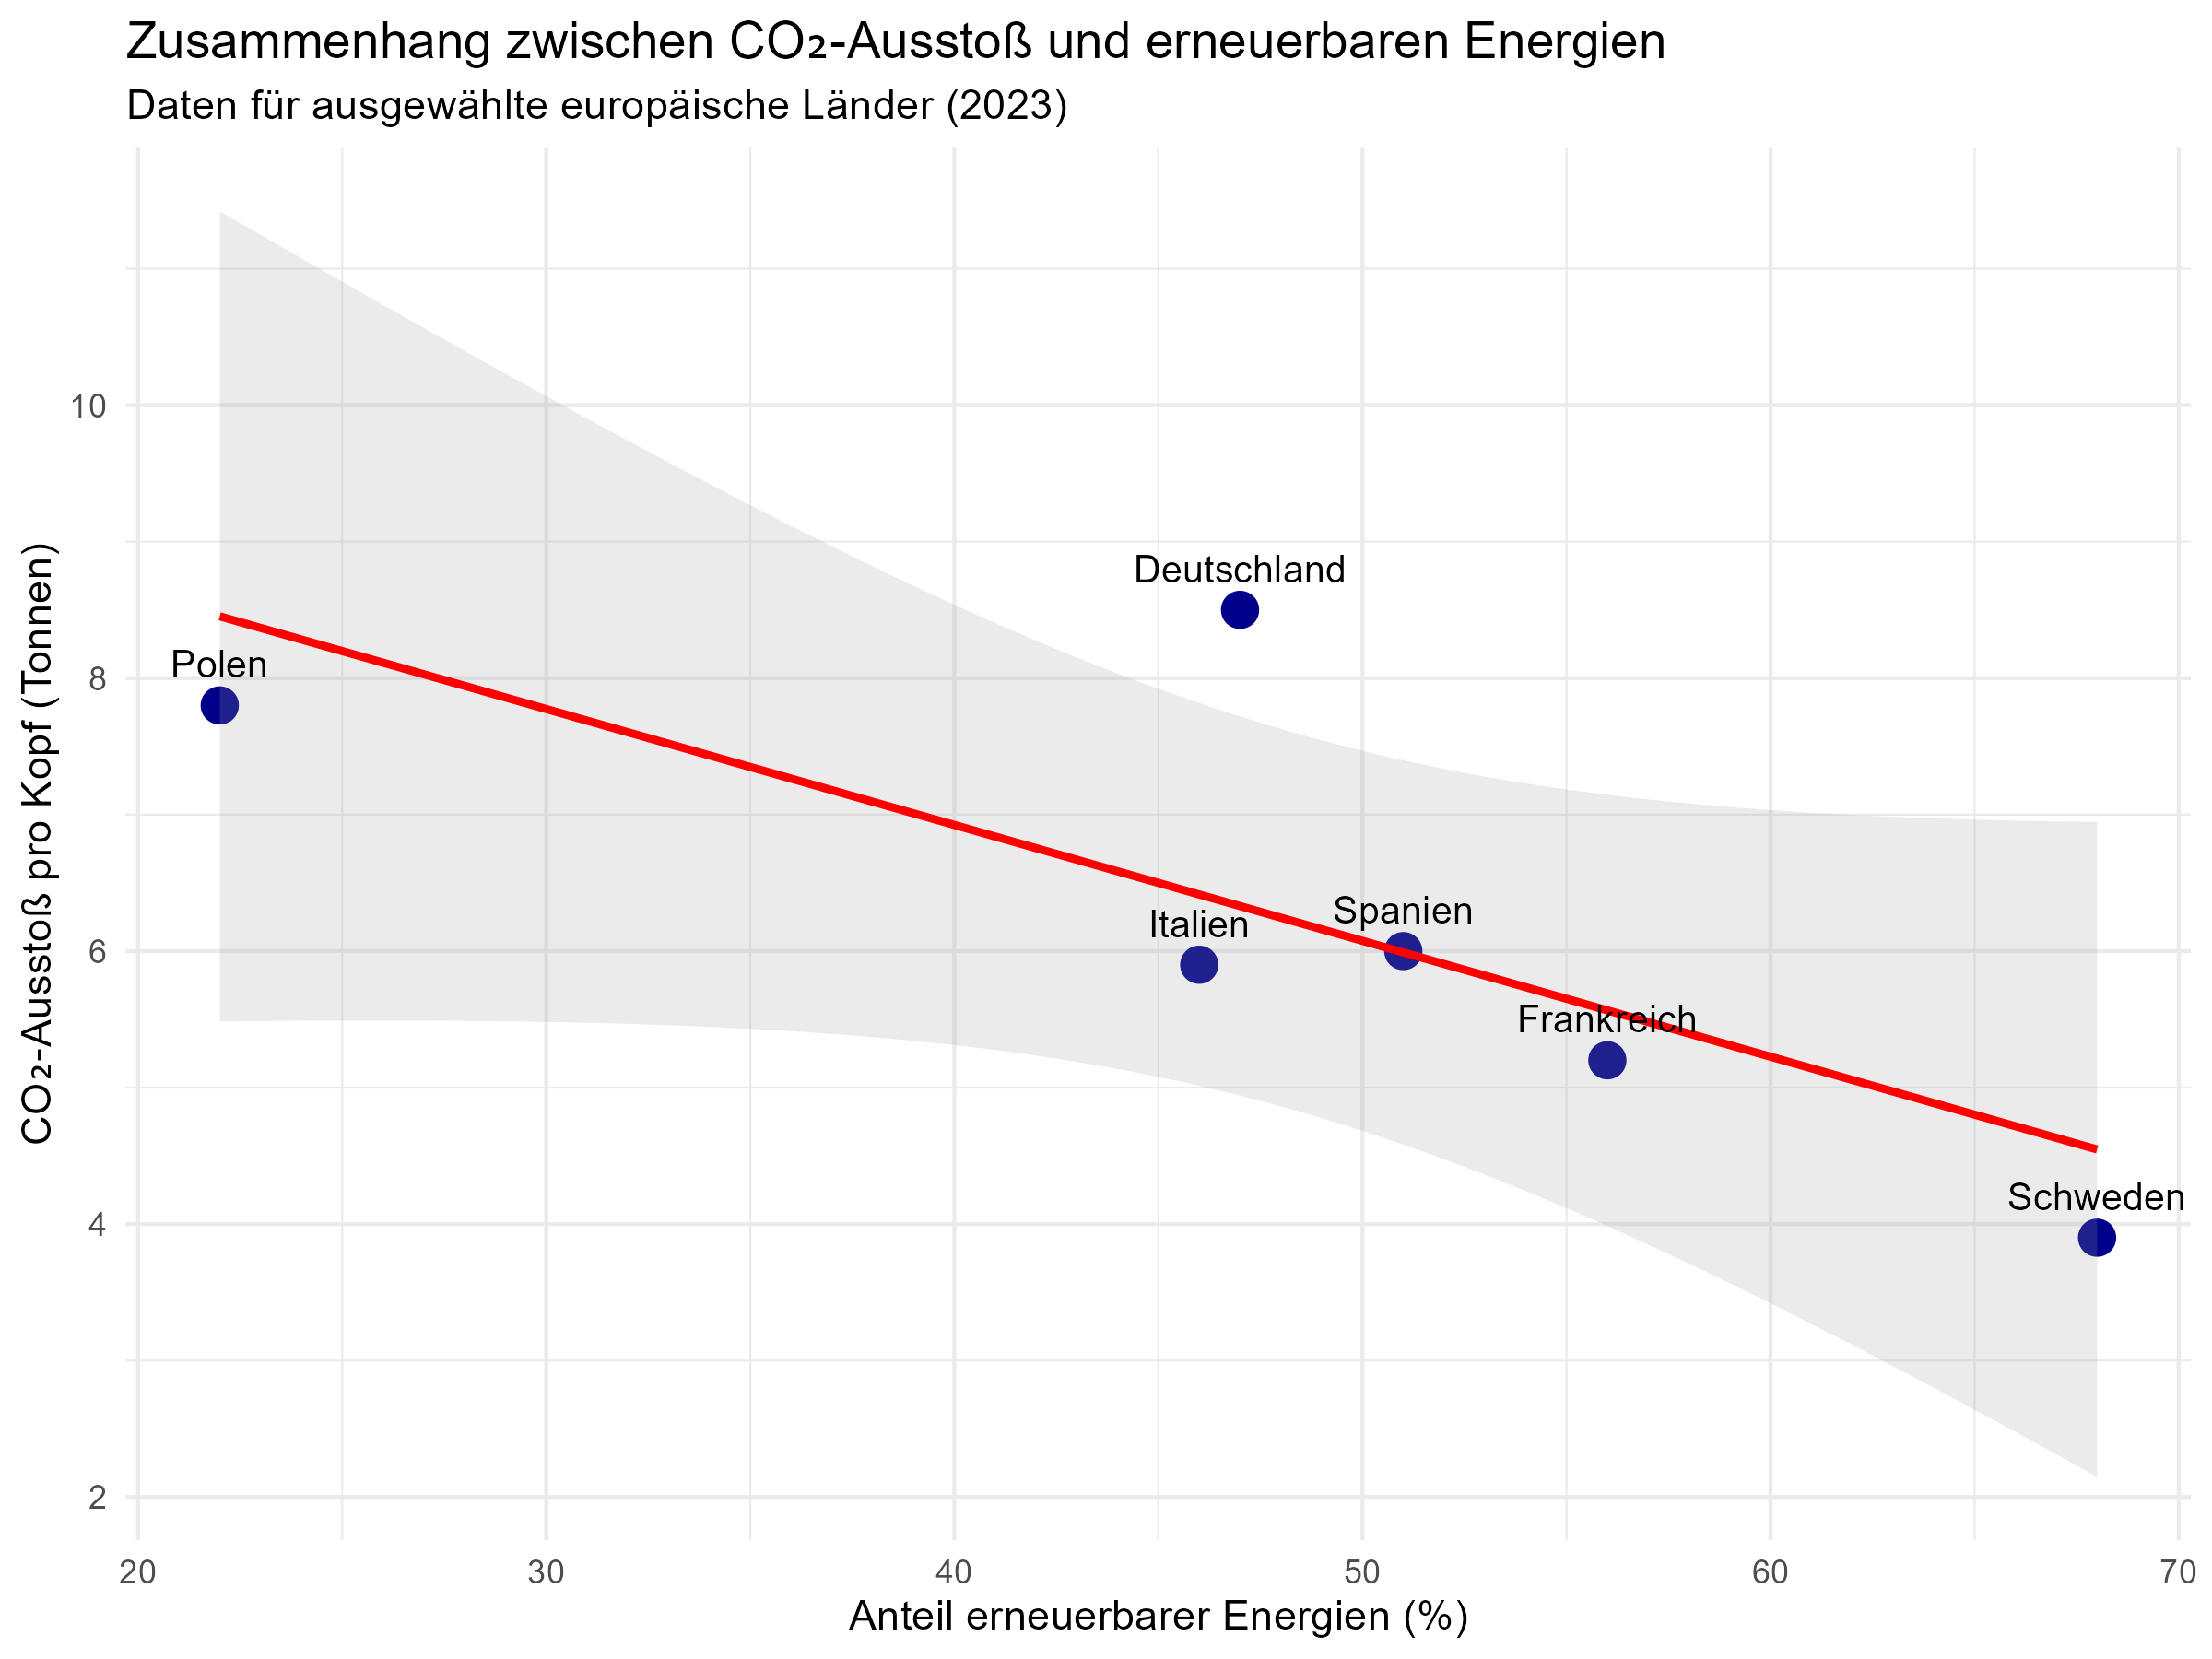
\includegraphics[keepaspectratio]{Aufgabe3c.png}}

\section{Fazit}\label{fazit}

Die Analyse zeigt einen negativen Zusammenhang zwischen dem Anteil
erneuerbarer Energien und dem CO2-Ausstoß pro Kopf.

\begin{center}\rule{0.5\linewidth}{0.5pt}\end{center}

\end{document}
